\documentclass[../Carre_nights.tex]{subfiles}

\begin{document}

\section{n0046}
\textbf{\Large{The tale of king Umar al-Num\=an and his two remarkable sons}} \\

\begin{figure}[ht]
\centering
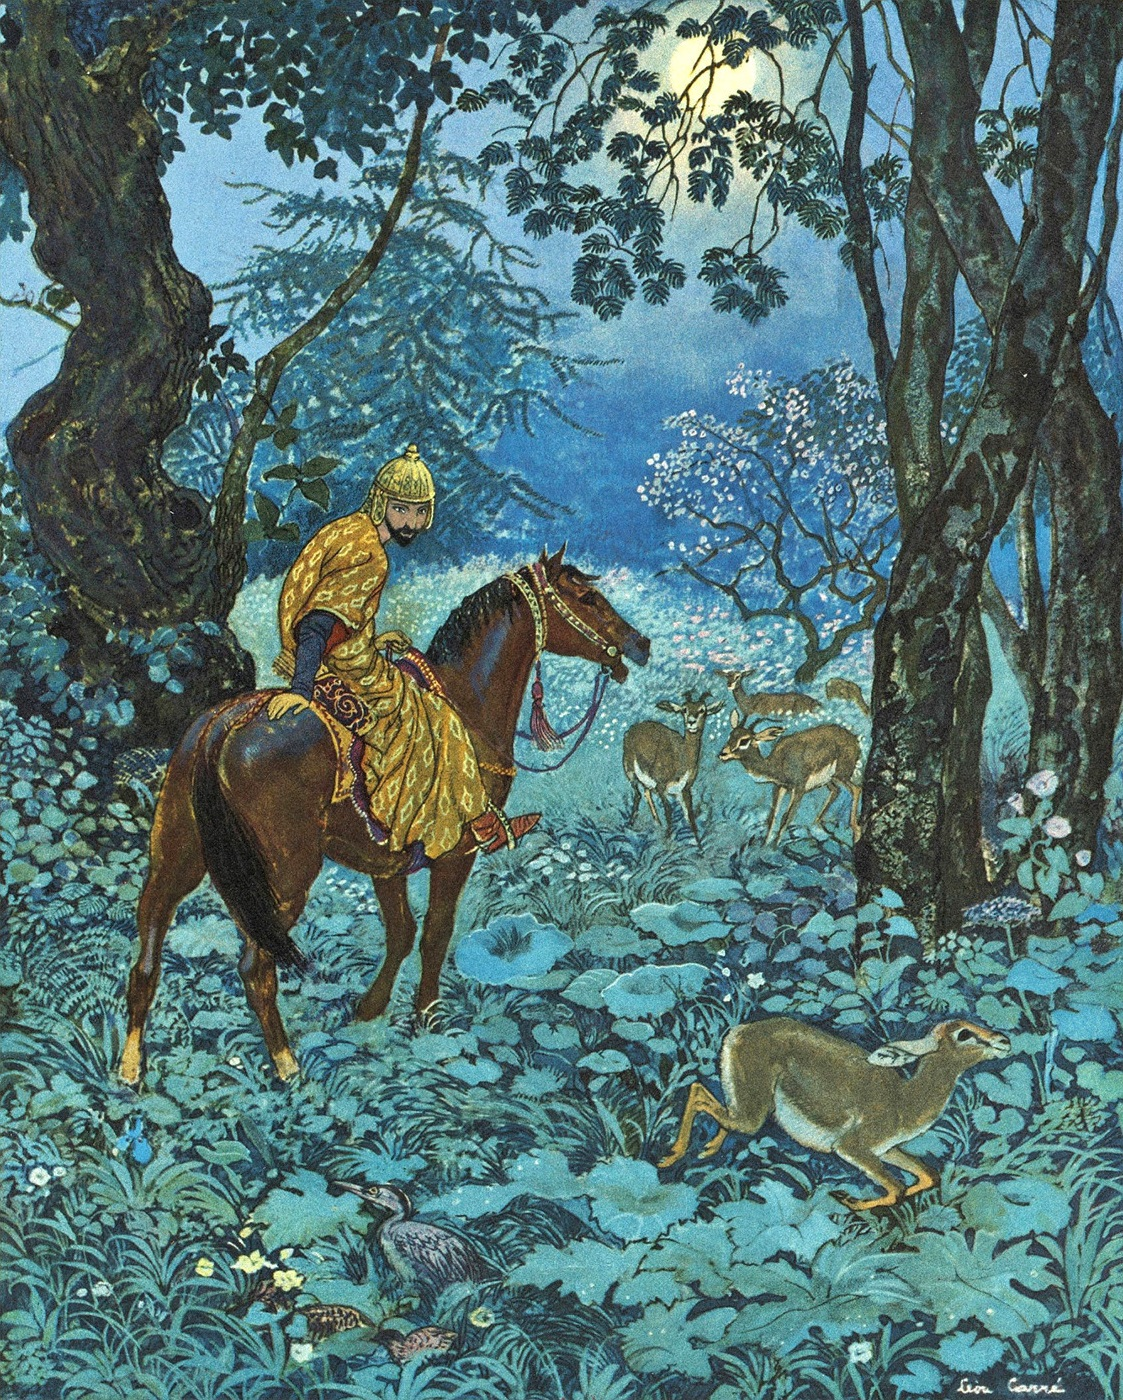
\includegraphics[height=\figsize]{illustrations/volume_2/T02, n0046 - Histoire du roi Omar Al-Némân et de ses deux fils merveilleux.jpg}
\end{figure}

\textit{\\
"Le cheval se mit ainsi à marcher jusqu’à minuit, et sou- dain, au milieu d’une solitude boisée, il s’arrêta et frappa violemment du sabot contre terre. Et Scharkân s’éveilla et se vit au milieu des arbres de la forêt, qui était en ce moment éclai- rée par la clarté de la lune. Et Scharkân fut extrêmement ému de se trouver au milieu de cet endroit solitaire..."} \\
—T02, n0046 - Histoire du roi Omar Al-Némân et de ses deux fils merveilleux \\~\\
\textit{"He was wakened at midnight by his horse pawing the ground violently and halting in the middle of a wooded solitude, brightly lighted by the moon. Shark\=an was startled to find himself in so lonely a place…"} \\
—V01, n0046 - The tale of king Umar al-Num\=an and his two remarkable sons

\newpage

\section{n0050}
\textbf{\Large{The tale of king Umar al-Num\=an and his two remarkable sons}} \\

\begin{figure}[ht]
\centering
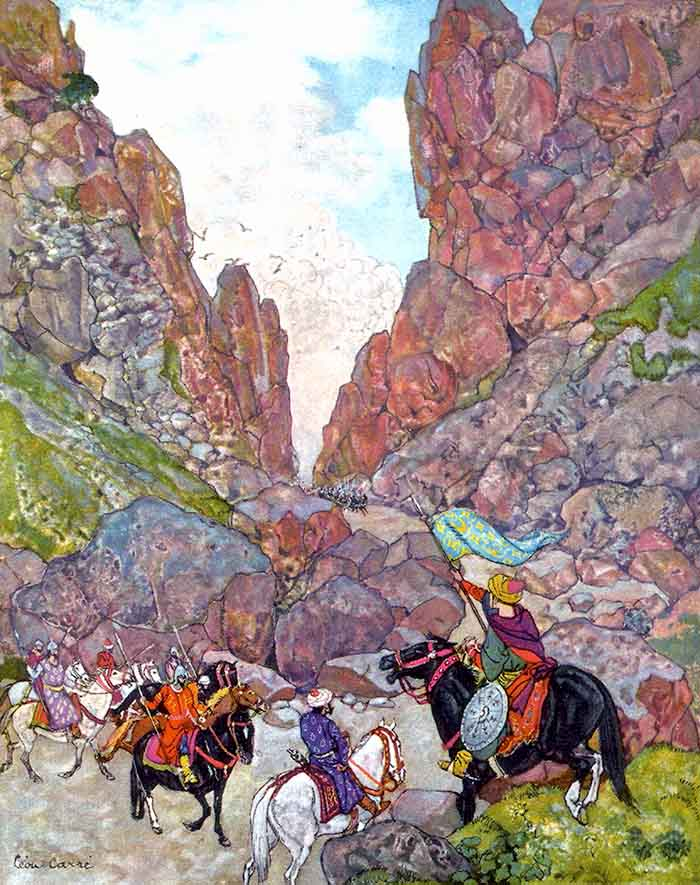
\includegraphics[height=\figsize]{illustrations/volume_2/T02, n0050 - Histoire du roi Omar Al-Némân et de ses deux fils merveilleux.jpg}
\end{figure}

\textit{\\
"...ils finirent par arriver à un défilé fort étroit situé entre deux très hautes montagnes. Et à peine y étaient-ils qu’ils virent à l’autre bout du défilé s’élever une poussière fort dense, qui se rapprocha rapidement et se dissipa pour laisser paraître cent cavaliers, disparaissant sous les cottes de mailles et les visières d’acier."} \\
—T02, n0050 - Histoire du roi Omar Al-Némân et de ses deux fils merveilleux \\~\\
\textit{"...they came to a narrow defile between two rocky hills, from the other end of which they saw a thick cloud of dust advancing. It came on rapidly and cleared as it approached, showing a hundred knights clad in coats of mail and vizors of steel…"} \\
—V01, n0050 - The tale of king Umar al-Num\=an and his two remarkable sons

\newpage

\section{n0053}
\textbf{\Large{The tale of king Umar al-Num\=an and his two remarkable sons}} \\

\begin{figure}[ht]
\centering
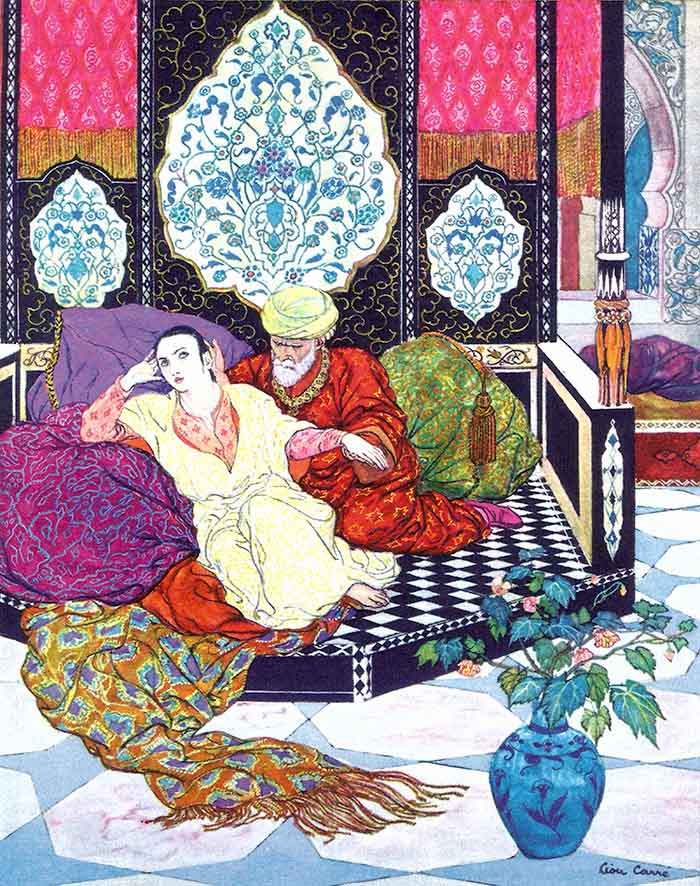
\includegraphics[height=\figsize]{illustrations/volume_2/T02, n0053 - Histoire du roi Omar Al-Némân et de ses deux fils merveilleux.jpg}
\end{figure}

\textit{\\
"...il s’attrista davantage de jour en jour et tellement, que le roi lui dit : « Qu’as-tu donc, ô mon fils, à jaunir de teint et à maigrir de corps ? »"} \\
—T02, n0053 - Histoire du roi Omar Al-Némân et de ses deux fils merveilleux \\~\\
\textit{"Day by day he became sadder, until at last Umar al-Num\=an noticed it and asked the reason for his sorrow."} \\
—V01, n0053 - The tale of king Umar al-Num\=an and his two remarkable sons

\newpage

\section{n0055}
\textbf{\Large{The tale of king Umar al-Num\=an and his two remarkable sons}} \\

\begin{figure}[ht]
\centering
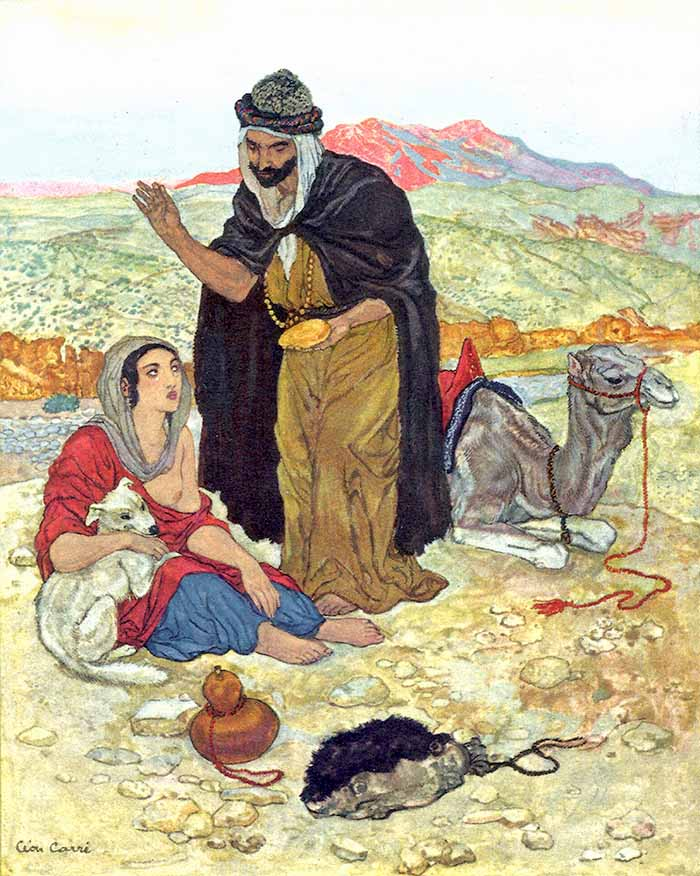
\includegraphics[height=\figsize]{illustrations/volume_2/T02, n0055 - Histoire du roi Omar Al-Némân et de ses deux fils merveilleux.jpg}
\end{figure}

\textit{\\
"...le Bédouin, qui adorait d’instinct la poésie, fut touché de pitié pour la belle malheureuse et il s’approcha d’elle et lui essuya les larmes et lui donna à manger une galette d’orge..."} \\
—T02, n0055 - Histoire du roi Omar Al-Némân et de ses deux fils merveilleux \\~\\
\textit{"...the Badaw\={\i}, who instinctively loved the sound of words, pitied the fair unfortunate, wiped her tears, and gave her a barley cake to eat..."} \\
—V01, n0055 - The tale of king Umar al-Num\=an and his two remarkable sons

\newpage

\section{n0067}
\textbf{\Large{The tale of king Umar al-Num\=an and his two remarkable sons}} \\

\begin{figure}[ht]
\centering
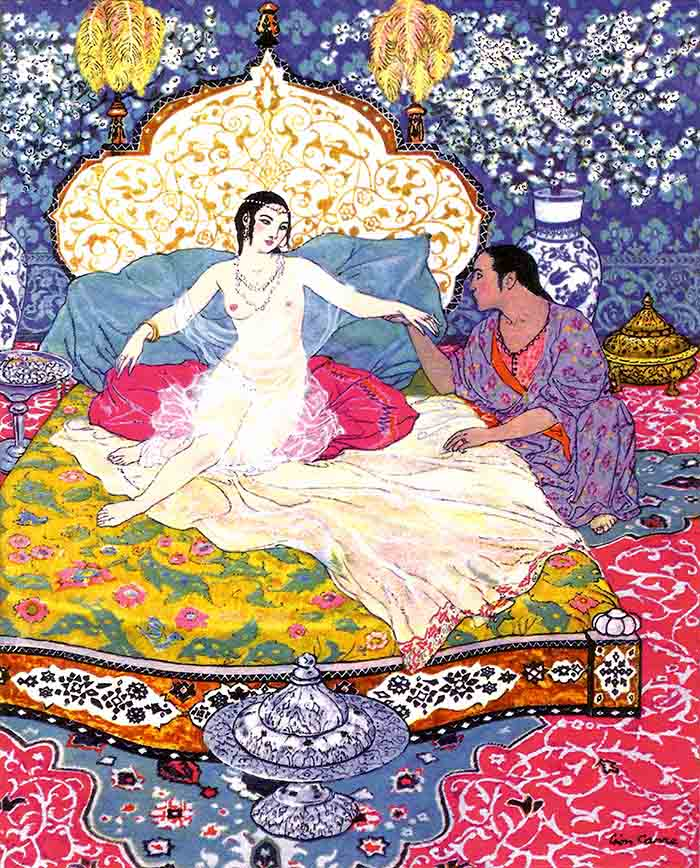
\includegraphics[height=\figsize]{illustrations/volume_2/T02, n0067 - Histoire du roi Omar Al-Némân et de ses deux fils merveilleux.jpg}
\end{figure}

\textit{\\
"...Scharkân fit son entrée dans la chambre nuptiale. Et il était loin de soupçonner que cette merveilleuse adolescente fût sa soeur Nôzhatou…"} \\
—T02, n0067 - Histoire du roi Omar Al-Némân et de ses deux fils merveilleux \\~\\
\textit{"When Shark\=n came to the couch, he was as ignorant that this beautiful girl was his sister..."} \\
—V01, n0067 - The tale of king Umar al-Num\=an and his two remarkable sons

\newpage

\section{n0078}
\textbf{\Large{The tale of king Umar al-Num\=an and his two remarkable sons [The tale of the death of king Umar al-Num\=an]}} \\

\begin{figure}[ht]
\centering
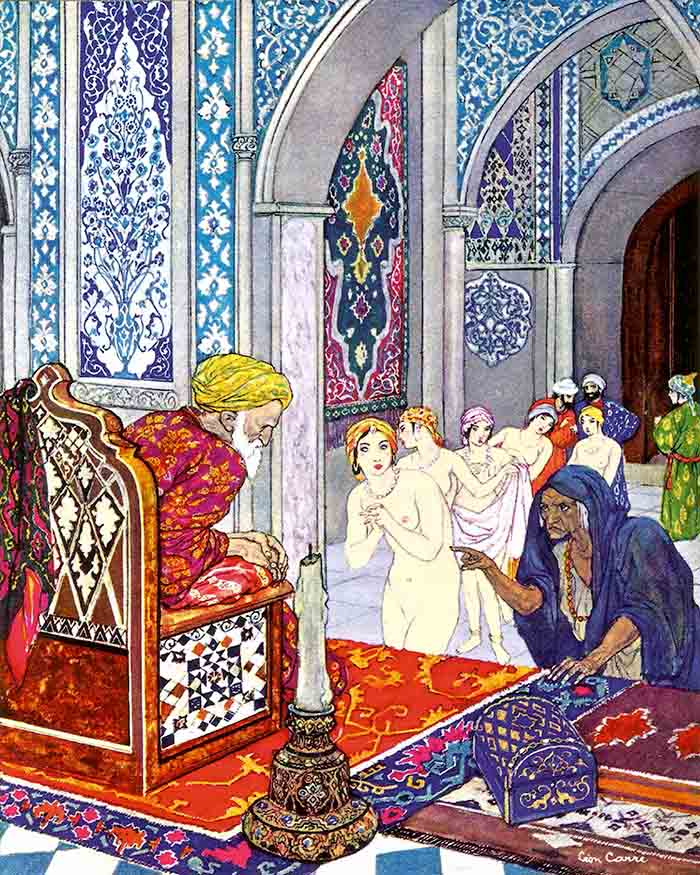
\includegraphics[height=\figsize]{illustrations/volume_2/T02, n0078 - Histoire du roi Omar Al-Némân et de ses deux fils merveilleux [Histoire de la mort du roi Omar Al-Némân].jpg}
\end{figure}

\textit{\\
"...la vénérable vieille s’avança entre les mains du roi et baisa la terre avec respect et dit : « Ô roi, voici que je t’apporte cinq joyaux que ne possède aucun roi de la terre. Et je te prie d’en examiner la beauté et de la mettre à l’épreuve ; car la beauté n’apparaît qu’à celui qui la cherche avec amour ! »"} \\
—T02, n0078 - Histoire du roi Omar Al-Némân et de ses deux fils merveilleux [Histoire de la mort du roi Omar Al-Némân] \\~\\
\textit{"The holy old lady kissed the earth between the King's hands, saying: 'I bring five jewels to you such as the court of no other king upon the earth has seen. I pray you to look upon their beauty and put them to the proof, for beauty is never apparent save to the search of love.'"} \\
—V01, n0078 - The tale of king Umar al-Num\=an and his two remarkable sons [The tale of the death of king Umar al-Num\=an]

\newpage

\section{n0094}
\textbf{\Large{The tale of king Umar al-Num\=an and his two remarkable sons}} \\

\begin{figure}[ht]
\centering
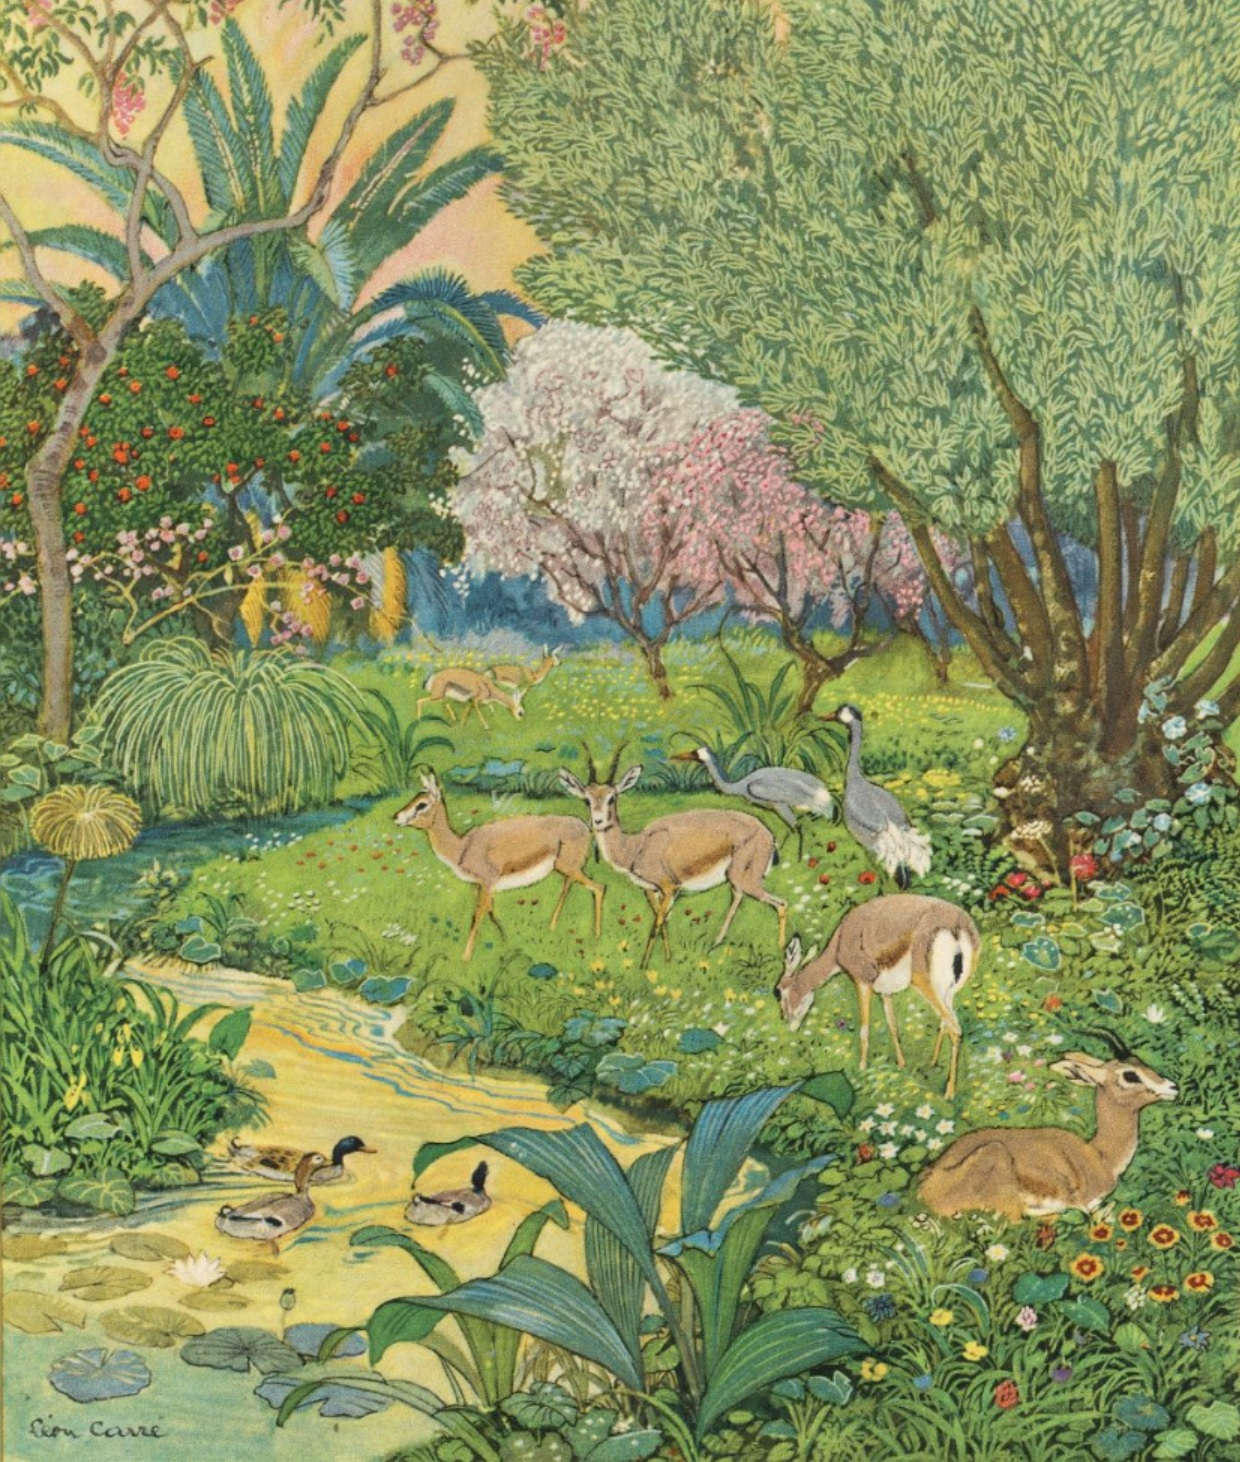
\includegraphics[height=\figsize]{illustrations/volume_2/T02, n0094 - Histoire du roi Omar Al-Némân et de ses deux fils merveilleux.jpg}
\end{figure}

\textit{\\
"...cette contrée, où s’ébattaient les gazelles et chantaient les oiseaux, apparaissait tel un paradis avec ses grands arbres ivres de la rosée, et ses fleurs qui souriaient à la brise..."} \\
—T02, n0094 - Histoire du roi Omar Al-Némân et de ses deux fils merveilleux \\~\\
\textit{"Birds sang there, gazelles leapt there, so that the place seemed some new Paradise, its great trees drunken with the dew upon their branches, and its flowers smiling to a vagabond south wind."} \\
—V01, n0094 - The tale of king Umar al-Num\=an and his two remarkable sons

\newpage

\section{n0108}
\textbf{\Large{The tale of king Umar al-Num\=an and his two remarkable sons}} \\

\begin{figure}[ht]
\centering
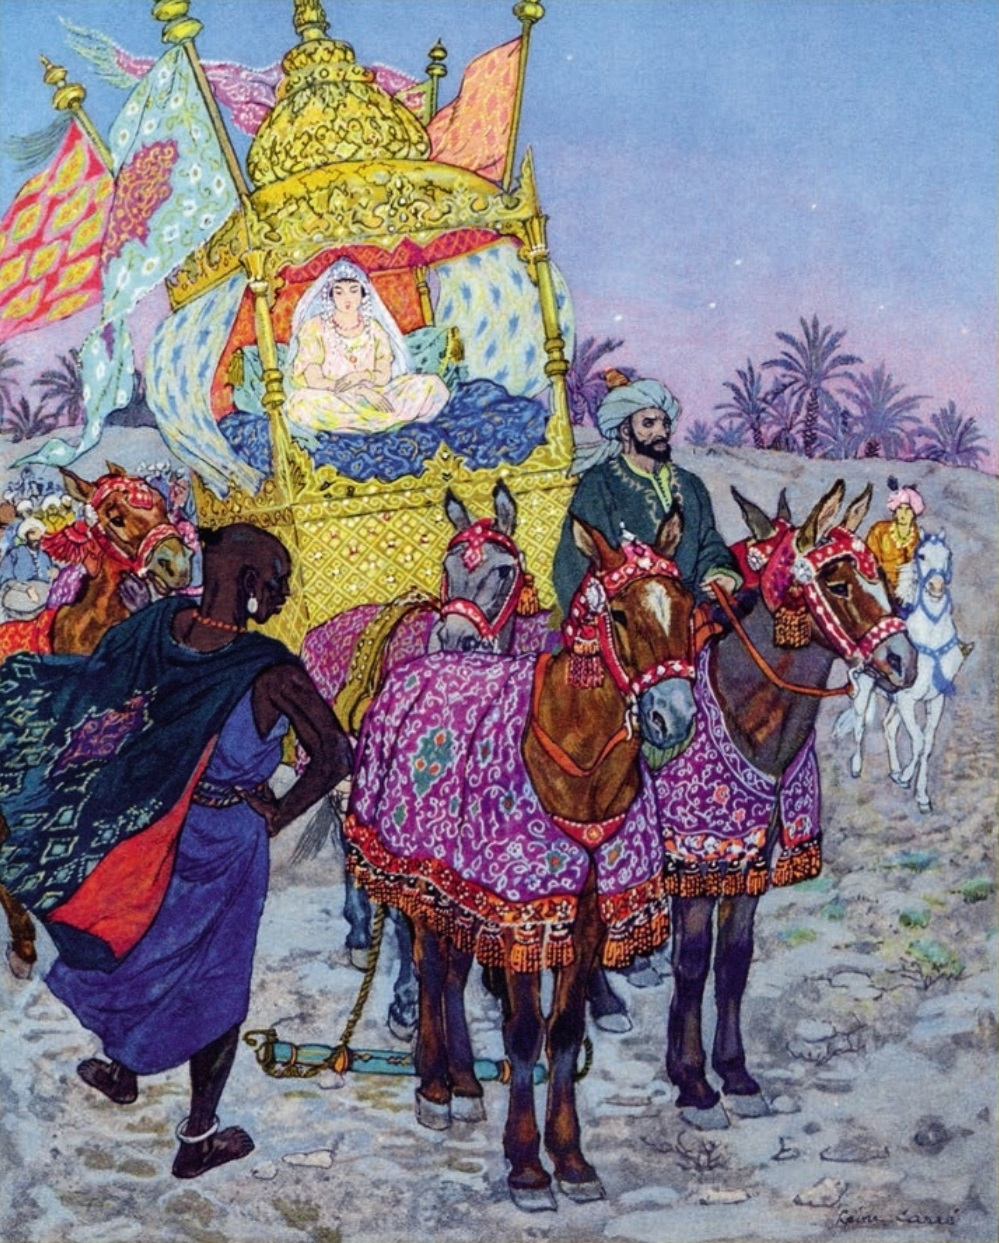
\includegraphics[height=\figsize]{illustrations/volume_2/T02, n0108 - Histoire du roi Omar Al-Némân et de ses deux fils merveilleux.jpg}
\end{figure}

\textit{\\
"...le palanquin apparaissait, dans la lueur du matin, tel un palais d’entre les palais des génies, et la jeune fille, couverte de ses voiles, telle une houria d’entre les plus belles hourias du paradis."} \\
—T02, n0108 - Histoire du roi Omar Al-Némân et de ses deux fils merveilleux \\~\\
\textit{"The convoy set out in the light of morning, the palanquin shining like a palace of fairies, and the veiled girl within it seeming like a h\=ur\={\i} sent from Paradise."} \\
—V01, n0108 - The tale of king Umar al-Num\=an and his two remarkable sons

\newpage

\section{n0116}
\textbf{\Large{The tale of Az\={\i}z and Az\={\i}zah [The tale of Az\={\i}z and Az\={\i}zah]}} \\

\begin{figure}[ht]
\centering
\includegraphics[height=\figsize]{illustrations/volume_2/T02, n0116 - Histoire d’Aziz et Aziza [Histoire du bel Aziz].jpg}
\end{figure}

\textit{\\
"...la première chose que je fis fut d’enlever le foulard de soie qui recouvrait le grand plateau d’argent. Et les choses délicieuses qui s’y trouvaient, je les vois encore devant mes yeux."} \\
—T02, n0116 - Histoire d’Aziz et Aziza [Histoire du bel Aziz] \\~\\
\textit{"I lifted the silk from the silver tray, and those delicacies which I found beneath I see even yet in my more happy dreams."} \\
—V01, n0116 - The tale of Az\={\i}z and Az\={\i}zah [The tale of Az\={\i}z and Az\={\i}zah]

\newpage

\section{n0129}
\textbf{\Large{The tale of Az\={\i}z and Az\={\i}zah [The tale of Az\={\i}z and Az\={\i}zah]}} \\

\begin{figure}[ht]
\centering
\includegraphics[height=\figsize]{illustrations/volume_2/T02, n0129 - Histoire d’Aziz et Aziza [Histoire du bel Aziz].jpg}
\end{figure}

\textit{\\
"...je vis entrer par la porte Sett-Donia, et je crus que la lune elle-même descendait dans le jardin. Sa beauté était telle que je restai cloué sur place, hébété, sans mouvement, mort."} \\
—T02, n0129 - Histoire d’Aziz et Aziza [Histoire du bel Aziz] \\~\\
\textit{"...I saw the lady Dunya come through the gate as if the moon herself were entering the garden. Such was her beauty that I remained where I was as if I had been dead."} \\
—V01, n0129 - The tale of Az\={\i}z and Az\={\i}zah [The tale of Az\={\i}z and Az\={\i}zah]

\newpage

\section{n0138}
\textbf{\Large{The tale of Az\={\i}z and Az\={\i}zah [The adventures of young K\=ana ma K\=ana]}} \\

\begin{figure}[ht]
\centering
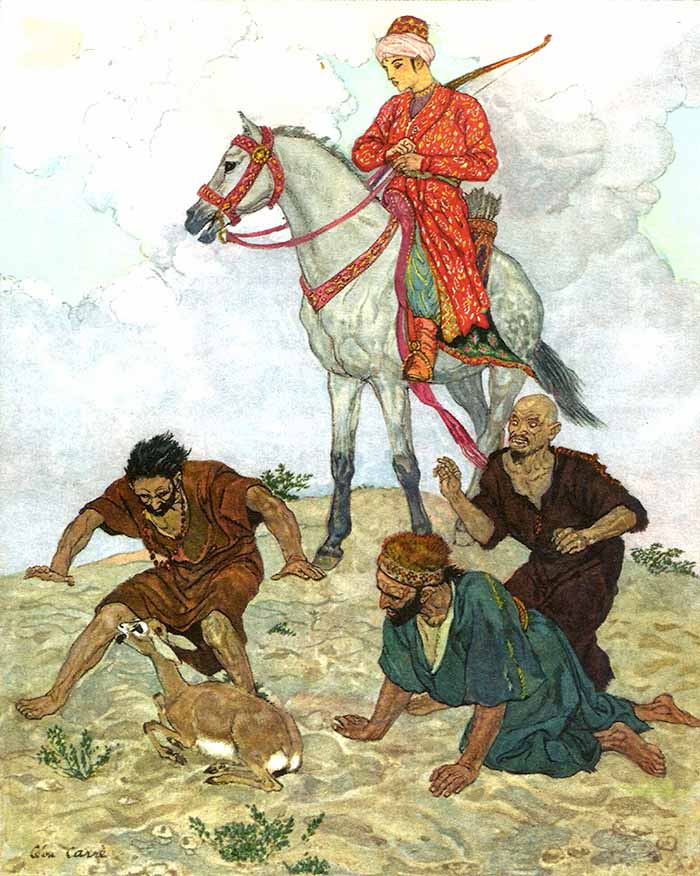
\includegraphics[height=\figsize]{illustrations/volume_2/T02, n0138 - Histoire d’Aziz et Aziza [Aventures de Kanmakân].jpg}
\end{figure}

\textit{\\
"Les exercices et la chasse, l’équitation et les joutes à la lance et au javelot, le tir à l’arc et les courses de chevaux avaient assoupli son corps et aguerri son âme. Et il était devenu le plus beau cavalier des pays musulmans..."} \\
—T02, n0138 - Histoire d’Aziz et Aziza [Aventures de Kanmakân] \\~\\
\textit{"Hunting and riding, tilting with the lance and javelin, shooting with the bow, and racing on horseback had suppled his body and fortified his spirit, until he had become the most accomplished cavalier to be found among the Faithful."} \\
—V01, n0138 - The tale of Az\={\i}z and Az\={\i}zah [The adventures of young K\=ana ma K\=ana]

\newpage

\section{n0141}
\textbf{\Large{The tale of Az\={\i}z and Az\={\i}zah [The adventures of young K\=ana ma K\=ana]}} \\

\begin{figure}[ht]
\centering
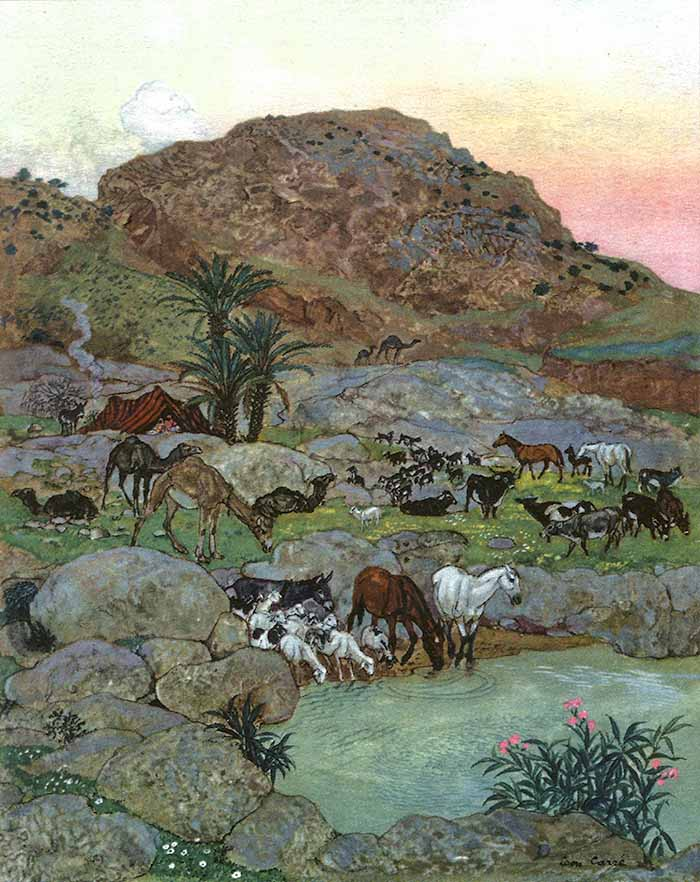
\includegraphics[height=\figsize]{illustrations/volume_2/T02, n0141 - Histoire d’Aziz et Aziza [Aventures de Kanmakân].jpg}
\end{figure}

\textit{\\
"...ils arrivèrent à une éminence au pied de laquelle s’étendait un pâtis couvert de chamelles et de chameaux, de moutons, de vaches et de chevaux. Et, plus loin, sous une tente, des esclaves armés étaient accroupis tranquillement."} \\
—T02, n0141 - Histoire d’Aziz et Aziza [Aventures de Kanmakân] \\~\\
\textit{"...they saw, at the bottom of the hill on which they sat, a pasture covered with camels and sheep, cattle and horses. A band of armed slaves sat under an awning and guarded the animals."} \\
—V01, n0141 - The tale of Az\={\i}z and Az\={\i}zah [The adventures of young K\=ana ma K\=ana]

\newpage

\section{n0146}
\textbf{\Large{The delightful tale of the beasts and birds [The tale of the goose]}} \\

\begin{figure}[ht]
\centering
\includegraphics[height=\figsize]{illustrations/volume_2/T02, n0146 - Histoire charmante des animaux et des oiseaux [Conte de l’oie].jpg}
\end{figure}

\textit{\\
"...c’était une île couverte de beaux arbres fruitiers et nourrie par une multitude de ruisseaux. Et le paon et son épouse furent extrêmement charmés de leur promenade au milieu de cette fraîcheur, et s’arrêtèrent quelque temps à manger de tous les fruits et à boire de cette eau si douce et si légère."} \\
—T02, n0146 - Histoire charmante des animaux et des oiseaux [Conte de l’oie] \\~\\
\textit{"They found the place covered with ripe fruit trees and nourished by a multitude of streams, so that they were charmed to walk about in the cool shadow and stop from time to time to eat the fruit and drink the clear water."} \\
—V01, n0146 - The delightful tale of the beasts and birds [The tale of the goose]

\newpage

\section{n0147}
\textbf{\Large{The delightful tale of the beasts and birds [The tale of the shepherd and the girl]}} \\

\begin{figure}[ht]
\centering
\includegraphics[height=\figsize]{illustrations/volume_2/T02, n0147 - Histoire charmante des animaux et des oiseaux [Le berger et l’adolescente].jpg}
\end{figure}

\textit{\\
"...la jeune fille se leva et, légère, se dévêtit entièrement et se tint droite et nue dans les flots de ses cheveux. Et l’appel de son silence, dans cette solitude de grotte, était plus terrible que tous les cris du délire."} \\
—T02, n0147 - Histoire charmante des animaux et des oiseaux [Le berger et l’adolescente] \\~\\
\textit{"The child rose and lightly undressed herself until she stood before him naked and white, bathed in the dark sea of her hair. Her silent invitation was more dangerous in that lonely cave than all the desirous cries which she had uttered before."} \\
—V01, n0147 - The delightful tale of the beasts and birds [The tale of the shepherd and the girl]

\newpage

\section{n0152}
\textbf{\Large{The tale of Al\={\i} ibn Bakr and the fair Shams al-Nah\=ar}} \\

\begin{figure}[ht]
\centering
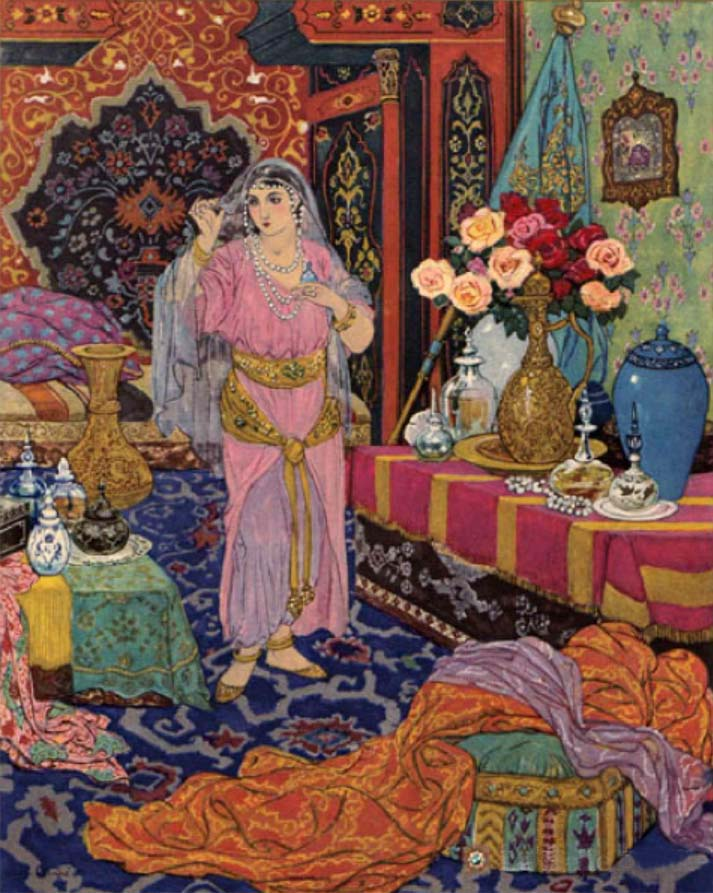
\includegraphics[height=\figsize]{illustrations/volume_2/T02, n0152 - Histoire d'Ali Ben-Bekar et de la belle Schamsennahar.jpg}
\end{figure}

\textit{\\
"...la jeune femme se mit à choisir négligemment quelques étoffes à fond d’or, quelques orfèvreries et quelques flacons d’essence de roses. Puis, comme elle n’avait pas à se gêner chez Abalhassan, elle releva un instant son petit voile de visage et fit ainsi briller, sans artifices, sa beauté."} \\
—T02, n0152 - Histoire d'Ali Ben-Bekar et de la belle Schamsennahar \\~\\
\textit{"She chose carelessly certain fabrics on a gold background, a few jewels, and some rare bottles of rose essence, lifting her veil the while to prove that she had no fear of the young merchant."} \\
—V01, n0152 - The tale of Al\={\i} ibn Bakr and the fair Shams al-Nah\=ar

\newpage

\section{n0155}
\textbf{\Large{The tale of Al\={\i} ibn Bakr and the fair Shams al-Nah\=ar}} \\

\begin{figure}[ht]
\centering
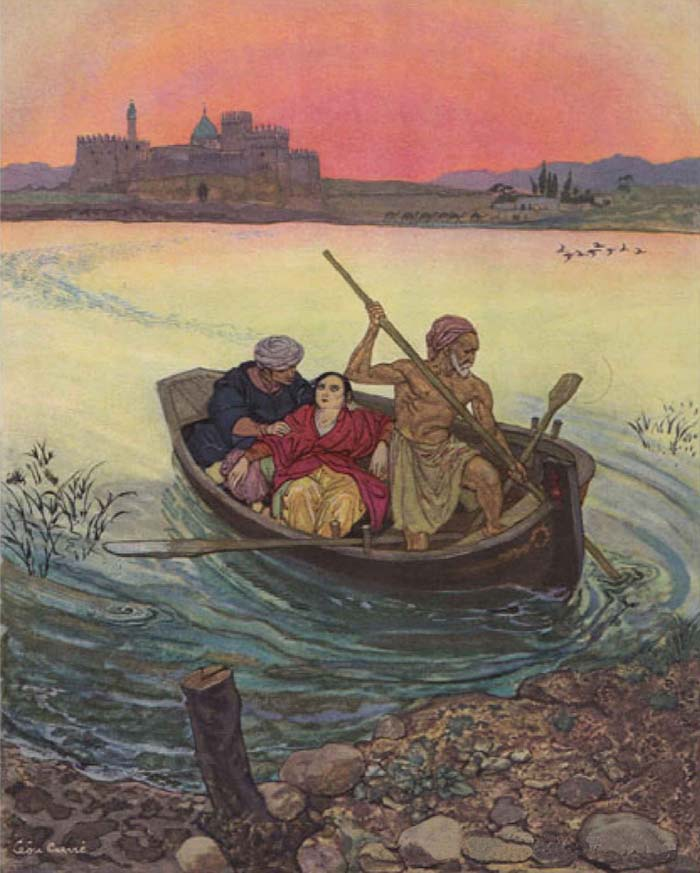
\includegraphics[height=\figsize]{illustrations/volume_2/T02, n0155 - Histoire d'Ali Ben-Bekar et de la belle Schamsennahar.jpg}
\end{figure}

\textit{\\
"...sans prononcer une parole, sur un simple signe de la confidente, il prit le prince Ali dans ses bras et le déposa dans l’embarcation, où ne tarda pas à entrer Abalhassan."} \\
—T02, n0155 - Histoire d'Ali Ben-Bekar et de la belle Schamsennahar \\~\\
\textit{"Without a word the oarsman took the prince in his arms and laid him down in the vessel. Ab\=u followed..."} \\
—V01, n0155 - The tale of Al\={\i} ibn Bakr and the fair Shams al-Nah\=ar

\newpage

\section{n0158}
\textbf{\Large{The tale of Al\={\i} ibn Bakr and the fair Shams al-Nah\=ar}} \\

\begin{figure}[ht]
\centering
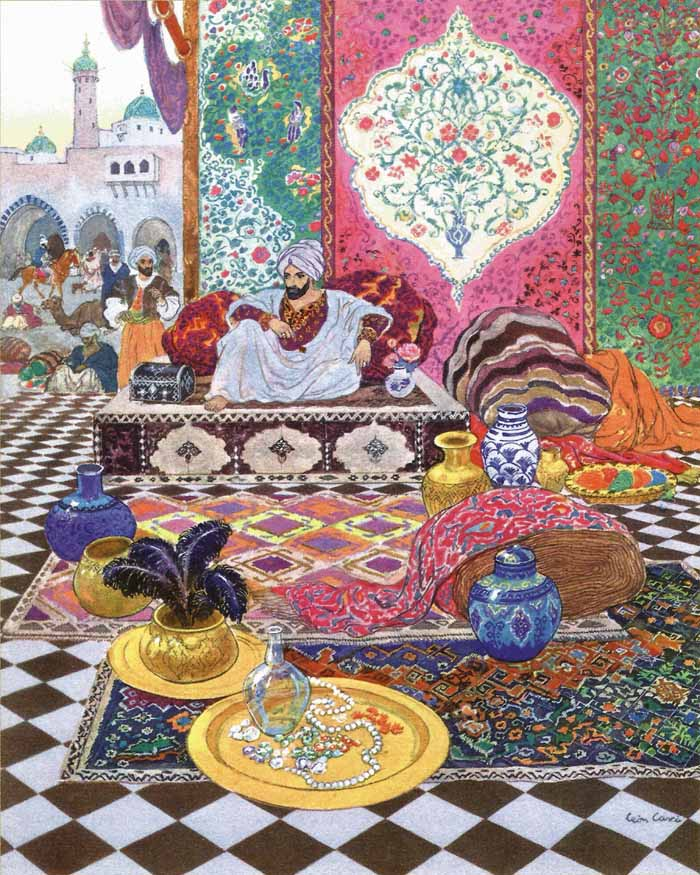
\includegraphics[height=\figsize]{illustrations/volume_2/T02, n0158 - Histoire d'Ali Ben-Bekar et de la belle Schamsennahar.jpg}
\end{figure}

\textit{\\
"...Abalhassan avait, parmi les amis qui le venaient voir le plus souvent, un jeune joaillier charmant, nommé Amin, et dont il avait pu souvent apprécier la discrétion. Et justement ce jeune joaillier vint en visite au moment même où, accoudé sur les coussins, Abalhassan était plongé dans la perplexité."} \\
—T02, n0158 - Histoire d'Ali Ben-Bekar et de la belle Schamsennahar \\~\\
\textit{"...the merchant numbered among his most intimate friends a certain young and discreet jeweller named Am\={\i}n, and this youth came to pay him a visit as he lay among his cushions trying to make up his mind what he should do."} \\
—V01, n0158 - The tale of Al\={\i} ibn Bakr and the fair Shams al-Nah\=ar

\newpage

\section{n0169}
\textbf{\Large{The tale of Al\={\i} ibn Bakr and the fair Shams al-Nah\=ar}} \\

\begin{figure}[ht]
\centering
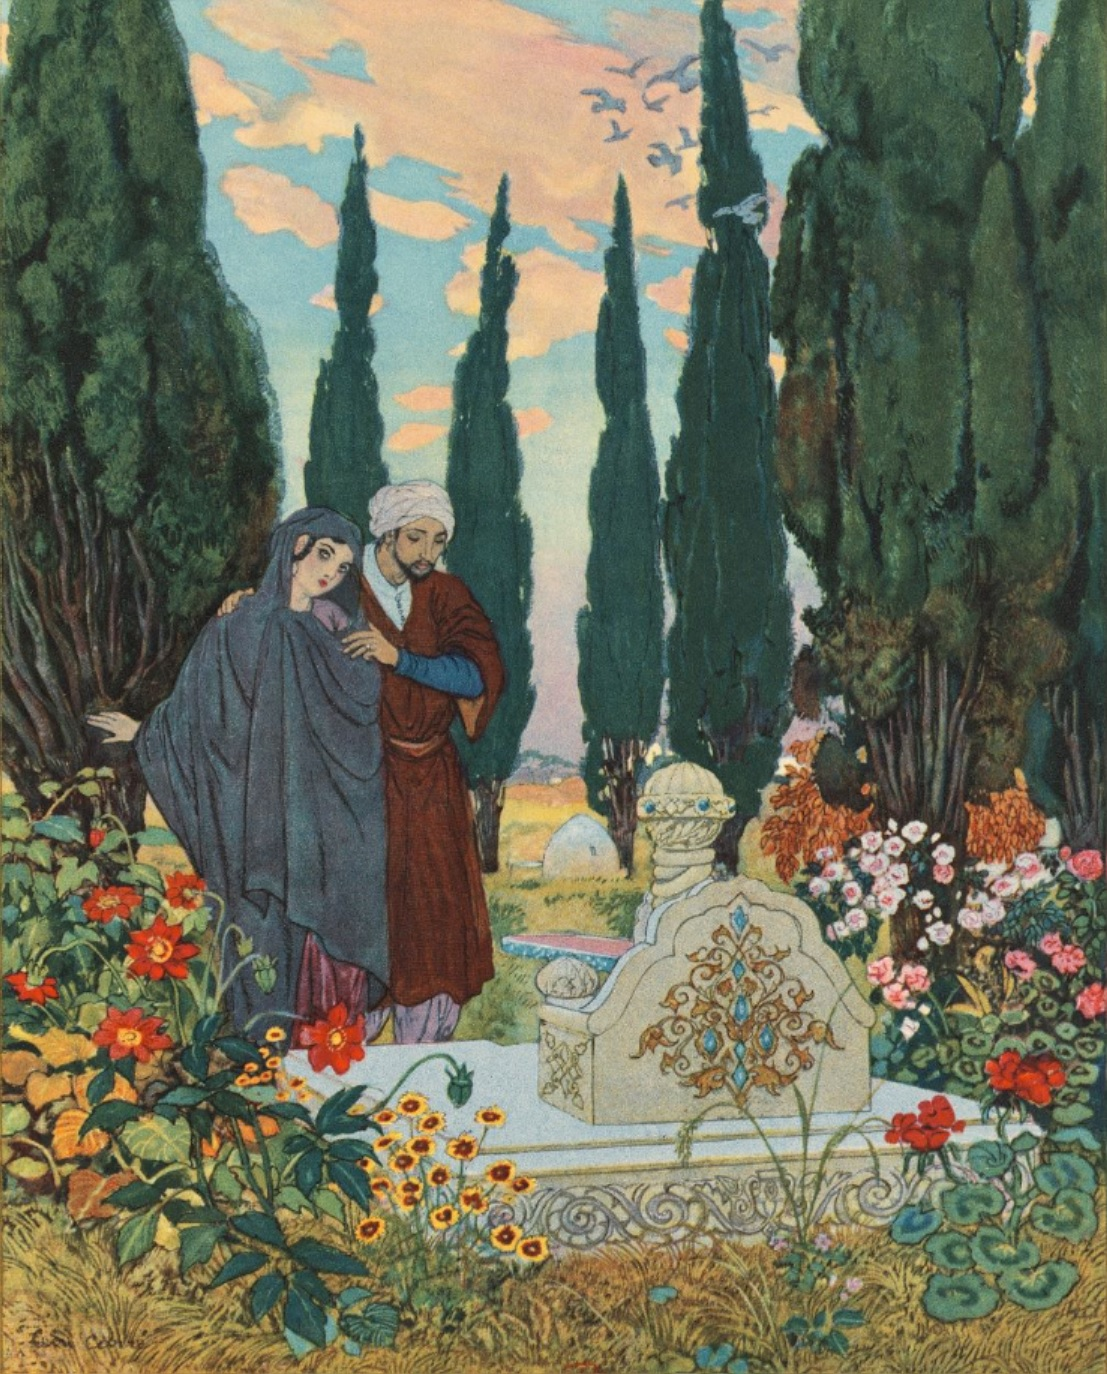
\includegraphics[height=\figsize]{illustrations/volume_2/T02, n0169 - Histoire d'Ali Ben-Bekar et de la belle Schamsennahar.jpg}
\end{figure}

\textit{\\
"...depuis lors ni moi ni la jeune fille, qui devint mon épouse, nous ne cessâmes d’aller visiter les deux tombeaux pour pleurer sur les amants dont nous avions été les amis."} \\
—T02, n0169 - Histoire d'Ali Ben-Bekar et de la belle Schamsennahar \\~\\
\textit{"Ever since then (concludes the jeweller) I and the confidant, who has become my wife, have not ceased at stated intervals to visit the two tombs and weep over the disastrous love of our young friends."} \\
—V01, n0169 - The tale of Al\={\i} ibn Bakr and the fair Shams al-Nah\=ar

\end{document}